\documentclass[letterpaper,11pt]{article}
\usepackage[utf8x]{inputenc}
\usepackage{enumerate}
\usepackage{enumitem}
\usepackage{fullpage}
\usepackage{amsmath}

\usepackage{pgf}
\usepackage{tikz}
\usepackage{circuitikz}
\usepackage{siunitx}

%opening
\title{Final Exam \\ Classical Mechanics \\ Physics 601 (Fall 2013)}
\date{Thursday December 12, 2013, 9am}

\begin{document}

\maketitle

\paragraph*{Instructions}
\begin{itemize}
 \item This exam is governed by \textbf{William \& Mary Honor Code}.
 \item This exam is to be completed \textbf{individually}.
 \item This exam is `open notes:' you are allowed to use the textbook, the posted lecture notes and homework solutions, and your personal notes.
 \item Carefully explain each step in your answer.
 \item Calculators are not needed for this exam.
 \item Write your \textbf{name on every page}.
 \item Write your responses on \textbf{single-sided} letter paper.
\end{itemize}

\pagebreak

\paragraph*{Lagrangian Mechanics}
\begin{enumerate}
 \item A point mass $m_1$ slides frictionlessly along a curve $y = f(x)$.  Assume $f(-x) = f(x)$ is an even function with a single minimum at $x = 0$, and that $f''(x) > 0$.  Affixed to the mass is a rigid rod of length $\ell$ with at the other end a second point mass $m_2$.  The entire system moves under the influence of gravity.  Choose as a set of generalized coordinates the set ${x,y,\theta}$, where $(x,y)$ are the Cartesian coordinates of the mass $m_1$, and $\theta$ is the angle between the rod and the downward vertical. [40 points]
 \begin{enumerate}
  \item Treat the condition $y = f(x)$ as a constraint.  Find four equations for the four unknowns $x$, $y$, $\theta$, and $\lambda$, where $\lambda$ is the Lagrange multiplier.  Without solving these equations, describe how you would determine the force of constraint normal to the wire. [10 points]
  \item Treat the system without the constraint formalism, using the generalized coordinates $x$ and $\theta$ only.  Find the Lagrangian $L(x,\theta,\dot{x},\dot{\theta},t)$.  Find the equilibrium values $(x^*,\theta^*)$ and determine the mass and potential matrices $M$ and $V$ (remember that $f(x)$ is an even function). [10 points]
  \item Consider the specific case $f(x) = x^2/2b$.  Define $\Omega_0 = \sqrt{g/b}$ and $\Omega_1 = \sqrt{g/\ell}$.  Find a general expression for the normal mode frequencies $\omega_\pm$.  Find the eigenvectors $z^\pm$ (you do not need to normalize them). [15 points]
  \item Find and interpret the limits of the frequencies $\omega_\pm$ for small $m_1$, and small $m_2$. [5 points]
  \begin{center}
   \begin{tikzpicture}[domain=-2.5:2.5]
    \draw[->] (-4.2,0) -- (4.2,0) node[right] {$x$};
    \draw[->] (0,-1.2) -- (0,2.8) node[left] {$y$};
    \draw plot[id=x] function{x*x*x*x/21} node[right] {$f(x)$};
    \filldraw (2,0.762) circle(3pt) node[right] {$m_1$};
    \begin{scope}[shift={(2,0.762)}]
     \draw (0,0) -- (-90:2);
     \draw (0,0) -- (-60:2);
     \draw[->] (0,0) -- (-90:1.2) arc (-90:-60:1.2) node[below left] {$\theta$};
     \filldraw (-60:2) circle (3pt) node[right] {$m_2$};
    \end{scope}
   \end{tikzpicture}
  \end{center}
 \end{enumerate}
\end{enumerate}

The coordinates of mass $m_1$ and $m_2$ are
\begin{eqnarray*}
 x_1 = x \quad & \quad & \quad x_2 = x + \ell \sin\theta, \\
 y_1 = y \quad & \quad & \quad y_2 = y - \ell \cos\theta.
\end{eqnarray*}
The time derivatives are then
\begin{eqnarray*}
 \dot{x}_1 = \dot{x} \quad & \quad & \quad \dot{x}_2 = \dot{x} + \ell \dot{\theta} \cos\theta, \\
 \dot{y}_1 = \dot{y} \quad & \quad & \quad \dot{y}_2 = \dot{y} + \ell \dot{\theta} \sin\theta.
\end{eqnarray*}
The Lagrangian is
\begin{eqnarray*}
 L & = & \frac{1}{2} m_1 (\dot{x}_1^2 + \dot{y}_1^2) + \frac{1}{2} m_2 (\dot{x}_2^2 + \dot{y}_2^2) - m_1 g y_1 - m_2 g y_2 \\
   & = & \frac{1}{2} (m_1 + m_2) (\dot{x}^2 + \dot{y}^2) + \frac{1}{2} m_2 \ell^2 \dot{\theta}^2 \\
   &   & + ~ m_2 \ell \dot{\theta} (\dot{x}\cos\theta + \dot{y}\sin\theta) \\
   &   & - ~ (m_1 + m_2) g y + m_2 g \ell \cos\theta.
\end{eqnarray*}
The equations of motion with the constraint $y - f(x) = 0$ and corresponding Lagrange multiplier $\lambda$ are
\begin{eqnarray*}
 (m_1 + m_2) \ddot{x} + m_2 \ell \ddot{\theta} \cos\theta - m_2 \ell \dot{\theta}^2 \sin\theta & = & - \lambda f'(x) \\
 (m_1 + m_2) \ddot{y} + m_2 \ell \ddot{\theta} \sin\theta + m_2 \ell \dot{\theta}^2 \sin\theta & = & \lambda - (m_1 + m_2) g \\
 m_2 \ell^2 \ddot{\theta} + m_2 \ell (\dot{x} \cos\theta + \dot{y} \sin\theta) - m_2 \ell \dot{\theta} (\dot{x} \sin\theta - \dot{y} \cos\theta) + m_2 g \ell \sin\theta & = & 0.
\end{eqnarray*}
After solving these equations, the reaction force $\vec{Q}$ normal to the curve is
\begin{equation*}
 \vec{Q} = - \lambda f'(x) \hat{e}_x + \lambda \hat{e}_y.
\end{equation*}

We can eliminate the constraint and obtain the Lagrangian
\begin{eqnarray*}
 L & = & \frac{1}{2} (m_1 + m_2) (1 + f'(x)^2) \dot{x}^2 + \frac{1}{2} m_2 \ell^2 \dot{\theta}^2 \\
   &   & + ~ m_2 \ell \dot{\theta} \dot{x} (\cos\theta + f'(x) \sin\theta) \\
   &   & - ~ (m_1 + m_2) g y + m_2 g \ell \cos\theta.
\end{eqnarray*}
The equilibrium is defined by
\begin{eqnarray*}
 \frac{\partial V}{\partial x} = f'(x) & = & 0, \\
 \frac{\partial V}{\partial \theta} = m_2 g \ell \sin\theta & = & 0,
\end{eqnarray*}
or $(x^*,\theta^*) = (0,0)$ because $f(x)$ has only a single minimum at $x = 0$.

The mass and potential matrices are
\begin{eqnarray*}
 M & = & \left[ \begin{array}{cc}
          \frac{\partial^2 L}{\partial \dot{x}^2} & \frac{\partial^2 L}{\partial \dot{x} \partial \dot{\theta}} \\
          \frac{\partial^2 L}{\partial \dot{x} \partial \dot{\theta}} & \frac{\partial^2 L}{\partial \dot{\theta}^2}
         \end{array} \right]_{x=0,\theta=0,\dot{x}=0,\dot{\theta}=0} \\
   & = & \left[ \begin{array}{cc}
          (m_1 + m_2) (1 + f'(x)^2) & m_2 \ell (\cos\theta + f'(x) \sin\theta) \\
           m_2 \ell (\cos\theta + f'(x) \sin\theta) & m_2 \ell^2
         \end{array} \right]_{x=0,\theta=0} \\
   & = & \left[ \begin{array}{cc}
          (m_1 + m_2) & m_2 \ell \\
           m_2 \ell & m_2 \ell^2
         \end{array} \right], \\
 V & = & \left[ \begin{array}{cc}
          \frac{\partial^2 V}{\partial x^2} & \frac{\partial^2 V}{\partial x \partial \theta} \\
          \frac{\partial^2 V}{\partial x \partial \theta} & \frac{\partial^2 V}{\partial \theta^2}
         \end{array} \right]_{x=0,\theta=0,\dot{x}=0,\dot{\theta}=0} \\
   & = & \left[ \begin{array}{cc}
          (m_1 + m_2) g f''(x) & 0 \\
          0 & m_2 g \ell
         \end{array} \right].
\end{eqnarray*}

For the specific parabolic function $f(x) = x^2/2b$ we find
\begin{eqnarray*}
  M & = & \left[ \begin{array}{cc}
          (m_1 + m_2) & m_2 \ell \\
           m_2 \ell & m_2 \ell^2
         \end{array} \right], \\
  V & = & \left[ \begin{array}{cc}
          (m_1 + m_2) \frac{g}{b} & 0 \\
          0 & m_2 g \ell
         \end{array} \right].
\end{eqnarray*}
The eigenvalue equation becomes, with $\Omega_0 = \sqrt{g/b}$ and $\Omega_1 = \sqrt{g/\ell}$,
\begin{equation*}
 \det (V - \omega^2 M) = \left| \begin{array}{cc}
          (m_1 + m_2) (\Omega_0^2 - \omega^2) & - m_2 \ell \omega^2 \\
           - m_2 \ell \omega^2 & m_2 \ell^2 (\Omega_1^2 - \omega^2)
         \end{array} \right| = 0.
\end{equation*}
The two solutions for this equations are
\begin{equation*}
 \omega_\pm^2 = \frac{m_1 + m_2}{m_1} \left[ \frac{\Omega_0^2 + \Omega_1^2}{2} \pm \sqrt{\left(\frac{\Omega_0^2 + \Omega_1^2}{2}\right)^2 + \frac{m_2}{m_1 + m_2} \Omega_0^2 \Omega_1^2} \right].
\end{equation*}
The eigenvectors are
\begin{eqnarray*}
 z_+ & = & \left[ \begin{array}{c}
                   1 \\
                   \frac{m_1 + m_2}{m_2} \left(\frac{\Omega_0^2}{\omega_+^2} - 1\right)
                  \end{array} \right], \\
 z_- & = & \left[ \begin{array}{c}
                   1 \\
                   \frac{m_1 + m_2}{m_2} \left(\frac{\Omega_0^2}{\omega_-^2} - 1\right)
                  \end{array} \right].
\end{eqnarray*}

For small $m_1$ we get
\begin{equation*}
 \omega_\pm^2 = \frac{m_2}{m_1} \left[ \frac{\Omega_0^2 + \Omega_1^2}{2} \pm \frac{\Omega_0^2 + \Omega_1^2}{2} \right].
\end{equation*}
The frequency $\omega_+$ corresponds to the pendulum motion of just $m_2$, while $\omega_-$ corresponds to the free motion of $m_1$ around the equilibrium without motion of $m_2$.

For small $m_2$ we get $\omega_+ = \Omega_0$ and $\omega_- = \Omega_1$, or $m_2$ oscillates independently as a pendulum would, and $m_1$ oscillates as a ball in a bowl would.


\paragraph*{Hamiltonian Mechanics}
\begin{enumerate}[resume]
 \item In the case of a time-dependent Hamiltonian $H\left(p,q;\lambda(t)\right)$ where the time-dependence is due to a parameter $\lambda$ that slowly varies in time, the action $J$ belongs to a class of observables known as \emph{adiabatic invariants}.  The change in $\lambda$ is said to be \emph{adiabatic} if the change $\Delta\lambda$ is slow compared to the period of the motion, or
 \begin{equation*}
  |\Delta\lambda| = |\dot\lambda| \Delta t = |\dot\lambda| \frac{2\pi}{\omega} \ll |\lambda|.
 \end{equation*}
 It can be shown that the action $J$ is \emph{conserved} for changes in the parameter $\lambda$ that satisfy this \emph{adiabatic condition}.

 At the first international Solvay congress in 1911, the following question was posed: how would the energy of a simple pendulum change if the length $\ell$ is changed slowly.  Model the simple pendulum with small amplitude as a harmonic oscillator $H\left(p,q;\omega(t)\right)$, and determine how the following quantities change when the length is \emph{doubled} adiabatically: [10 points]
 \begin{itemize}
  \item the total energy $E$ of the harmonic oscillator,
  \item the amplitude $\theta_{max}$ of the pendulum.
 \end{itemize}
\end{enumerate}

The action variable for a harmonic oscillator is $J = E/\omega$.  If the action is constant, $J' = J$, then the energy has to change as the frequency $\omega' = \sqrt\frac{g}{\ell'}$ and a doubling of the length $\ell' = 2 \ell$ will result in a reduction of the energy by $\sqrt{2}$ to $E' = E / \sqrt{2}$.  The amplitude $\theta_{max}$ is related to the energy by
\begin{equation*}
 E = \frac{1}{2} m\ell^2\theta_{max}^2,
\end{equation*}
or
\begin{equation*}
 \theta_{max} = \sqrt{\frac{2 E}{m\ell^2}}.
\end{equation*}
The new amplitude is now
\begin{equation*}
 \theta_{max}' = \sqrt{\frac{2 E'}{m\ell'^2}} = \sqrt{\frac{2 E}{4\sqrt{2}m\ell^2}} = \frac{1}{2\sqrt{\sqrt{2}}} \theta_{max}.
\end{equation*}


\paragraph*{Small Oscillations}
\begin{enumerate}[resume]
 \item Consider the following coupled $LC$ circuit where $I_{1,2} = dQ_{1,2}/dt$ is the current flowing in a loop of the circuit, $L$ is the inductance of the inductor, and $C$ is the capacitance of the capacitor.  By analogy to mechanical oscillators, the inductance plays the role of an inertial mass, the capacitance plays the role of a spring constant.  The kinetic energy in an inductor is $\frac{1}{2} L I^2$, the potential energy in a capacitor is $\frac{1}{2 C} Q^2$.  The voltage across an inductor is $L \frac{d I}{d t}$, the voltage across a capacitor is $Q/C$.
 \begin{center}
  \begin{circuitikz}
   \draw (0,3) to (4,3);
   \draw (0,0) to[L, i=$I_1$, l=$L$] (0,3);
   \draw (0,0) to[C, l=$C$] (2,0);
   \draw (2,0) to[C, l=$C$] (4,0);
   \draw (4,0) to[L, i=$I_2$, l=$L$] (4,3);
   \draw (2,0) to (2,1);
   \draw (2,3) to[C, l=$C$] (2,1);
  \end{circuitikz}
 \end{center}
 \begin{enumerate}
  \item Determine the Lagrangian for this circuit, and show that the correct Kirchhoff equations can indeed be derived. [10 points]
  \item Treating the Lagrangian\footnotemark{} as a small oscillations problem, what are the frequencies of oscillation and the normal modes for this circuit when the currents and charges are small? [10 points]
  \footnotetext{For partial credit, use this \emph{incorrect} Lagrangian $L(I_1,I_2,Q_1,Q_2) = \frac{1}{2} L (I_1^2 + I_2^2) - \frac{1}{2 C} \left(Q_1 + Q_2\right)^2$}
 \end{enumerate}
\end{enumerate}

The Lagrangian for the system is
\begin{equation*}
 L = \frac{1}{2} L (I_1^2 + I_2^2) - \frac{1}{2 C} \left(Q_1^2 + Q_2^2 + (Q_1 + Q_2)^2\right).
\end{equation*}
The equations of motion are
\begin{eqnarray*}
 L \dot{I}_1 + \frac{1}{C} Q_1 + \frac{1}{C} (Q_1 + Q_2) & = & 0, \\
 L \dot{I}_2 + \frac{1}{C} Q_2 + \frac{1}{C} (Q_1 + Q_2) & = & 0.
\end{eqnarray*}
These are indeed the Kirchhoff equations one would find for the left loop and the right loop.

We can write the Lagrangian in matrix form with the mass matrix $M$ and the potential matrix $V$,
\begin{eqnarray*}
 M & = & L \left[ \begin{array}{cc}
            1 & 0 \\ 0 & 1
           \end{array} \right], \\
 V & = & \frac{1}{C} \left[ \begin{array}{cc}
            2 & 1 \\ 1 & 2
           \end{array} \right].
\end{eqnarray*}
The eigenvalue equation $\det(V - \omega^2 M) = 0$ becomes
\begin{equation*}
 \left| \begin{array}{cc}
  2 - \omega^2 L C & 1 \\ 1 & 2 - \omega^2 L C
 \end{array} \right| = 0,
\end{equation*}
or $(2 - \omega^2 LC)^2 = 1$.  The solutions of this equation are
\begin{eqnarray*}
 \omega_+^2 & = & \frac{1}{LC}, \\
 \omega_-^2 & = & \frac{3}{LC}.
\end{eqnarray*}
The eigenvectors are
\begin{eqnarray*}
 z_+ & = & \left[ \begin{array}{c} 1 \\ -1 \end{array} \right], \\
 z_- & = & \left[ \begin{array}{c} 1 \\ 1 \end{array} \right].
\end{eqnarray*}
We normalize these eigenvectors with the mass matrix $M$ and get
\begin{eqnarray*}
 \tilde{z}_+ & = & \frac{1}{\sqrt{2L}} \left[ \begin{array}{c} 1 \\ -1 \end{array} \right], \\
 \tilde{z}_- & = & \frac{1}{\sqrt{2L}} \left[ \begin{array}{c} 1 \\ 1 \end{array} \right].
\end{eqnarray*}
The normal modes $\xi$ are then
\begin{eqnarray*}
 \left[ \begin{array}{c} \xi_+ \\ \xi_- \end{array} \right] & = & U^T  \left[ \begin{array}{c} I_1 \\ I_2 \end{array} \right] \\
 & = & \frac{1}{\sqrt{2L}} \left[ \begin{array}{cc} 1 & 1 \\ -1 & 1 \end{array} \right]^T  \left[ \begin{array}{c} I_1 \\ I_2 \end{array} \right] \\
 & = & \frac{1}{\sqrt{2L}} \left[ \begin{array}{cc} 1 & -1 \\ 1 & 1 \end{array} \right]  \left[ \begin{array}{c} I_1 \\ I_2 \end{array} \right] \\
 & = & \frac{1}{\sqrt{2L}} \left[ \begin{array}{c} I_1 - I_2 \\ I_1 + I_2 \end{array} \right].
\end{eqnarray*}


\paragraph*{Rigid Bodies}
\begin{enumerate}[resume]
 \item Consider a ``rolling top'' that consists of two identical solid metal spheres of radius $R$ that are point-welded together.
 \begin{center}
  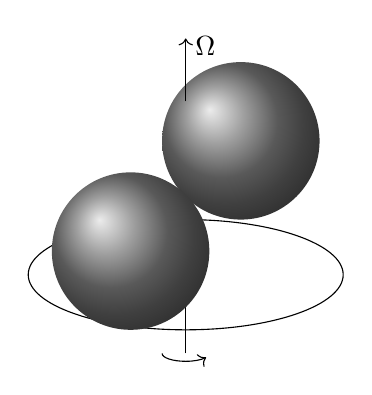
\begin{tikzpicture}
   \draw (-0.3,-2)[->] arc (180:330:0.3 and 0.1);
   \draw (0,-1) ellipse (2 and 0.7);
   \shade[ball color=gray] ( 0.7, 0.7) circle (1);
   \draw (0,-2) -- (0,0);
   \draw (0,1.2)[->] -- (0,2) node[very near end,right] {$\Omega$};
   \shade[ball color=gray] (-0.7,-0.7) circle (1);
  \end{tikzpicture}
 \end{center}
 Determine the principal moments of inertia of this top with respect to the center of mass. [10 points]
\end{enumerate}

The moment of inertia of a single sphere around the center is $\frac{2}{5} M R^2$.  The parallel axis theorem tells us that the moments of inertia of a sphere around the intersection of the $\hat{e}_z$ axis and the surface will be $I_1 = I_2 = \frac{2}{5} M R^2$ and $I_3 = \frac{2}{5} M R^2 + M R^2 = \frac{7}{5} M R^2$.  For two spheres this becomes $I_1 = I_2 = \frac{4}{5} M R^2$ and $I_3 = \frac{14}{5} M R^2$.

\end{document}
